\documentclass[a4paper]{article}

\usepackage[english]{babel}
\usepackage[utf8]{inputenc}
\usepackage{amsmath,amsfonts}
\usepackage{graphicx}
\usepackage[colorinlistoftodos]{todonotes}
\usepackage[margin=1in]{geometry}
\usepackage{enumitem}
\usepackage{multirow}
\usepackage{graphicx,wrapfig,lipsum}
\usepackage{graphicx} % for images
\usepackage{caption} % for captions under images/figures
\usepackage{url} % for urls


\setcounter{tocdepth}{5}
\setcounter{secnumdepth}{5}

\title{CS 669 Assignment 2}

\author{Rohit Patiyal \\ Devang Bacharwar \\ Mani Kumar}

\date{\today}

\begin{document}


\maketitle

\vspace{2.0cm}

\tableofcontents

\clearpage

\section {Objective}
	To build bayes classifier using Gaussian Mixture Model. Gaussian Mixture Model
	is built using the K-means clustering to initialize the parameters. The
	following data sets are used :
	\begin{enumerate}
		\item{2-D artificial Data of 3 or 4 classes that are nonlinearly
		separable.}
			
		\item{Real world data of 3 classes: The real world data sets correspond to
			  the formant frequencies F1 and F2 for vowel utterances.}
		\item{Scene image data corresponding to 3 different classes 
			A 23-dimensional feature vector is extracted from local blocks of an image for
	a particular scene. The 23-dimensional features include color histogram, edge
	directed histograms and entropy of wavelet coefficients. Each scene image is represented as a collection of 23-dimensional local feature vectors. 
	Each file in a folder of a class indicates a scene image.}
	\end{enumerate}
	
		
\vspace{1.0cm}

\section{Procedure}
	\begin{enumerate}
	  \item {Data for each class is partitioned into 75 \% for training and 25
	  \% for testing }
	  \item {The Data Set of each class is assumed to be Gaussian distribution
	  but with multimodes. Now the distribution is assumed to be a mixture of
	  $k$ Gaussian distributions}
	  \item {Mean, Covariances and mixing coefficients are initialized for each
	  of the mixtures for a class using k-means clustering, using the training
	  data. Different values of k are taken. k $\epsilon$ \{ 2, 4, 8, $\cdots$ \} }
	  \item {Starting from the initialized parameters from k-means, Means,
	  Covariances and mixing coefficients for each mixture are estimated by
	  maximizing the log likelihood which works on the optimization technique
	  Expectation Maximization.}
	  \item {For points in a grid, likelihood is calculated for each class and is
	  labeled as of the class with the maximum likelihood probability.}
      \item {Labels for test data are calculated and confusion matrix with '/.}
	  \item {These labelled points are plotted with different colors to visualize
	  the different regions separated by the decision boundaries.}
	  \item {The training data is also plotted over the regions, and observations
	  are made.}
	\end{enumerate}

\vspace{1.0cm}


\section{Observations}
	Here the cluster components are with respect to each class.The assumption taken is that each class have same number of cluster components.
	\subsection{Interlock Data Set}
    Interlock dataset has two classes with different means and similar covariances.
    
       \subsubsection{2 clusters components}
       2 clusters per each class gives 4 gaussian distribution which have spreads in different directions. The upper peak on the distribution determines the class for that region so giving out 4 intersection decision boundaty surfaces for gaussian distributions.
       
		\begin{minipage}[t]{0.6\linewidth}
			\vspace{0pt} % [3]
			 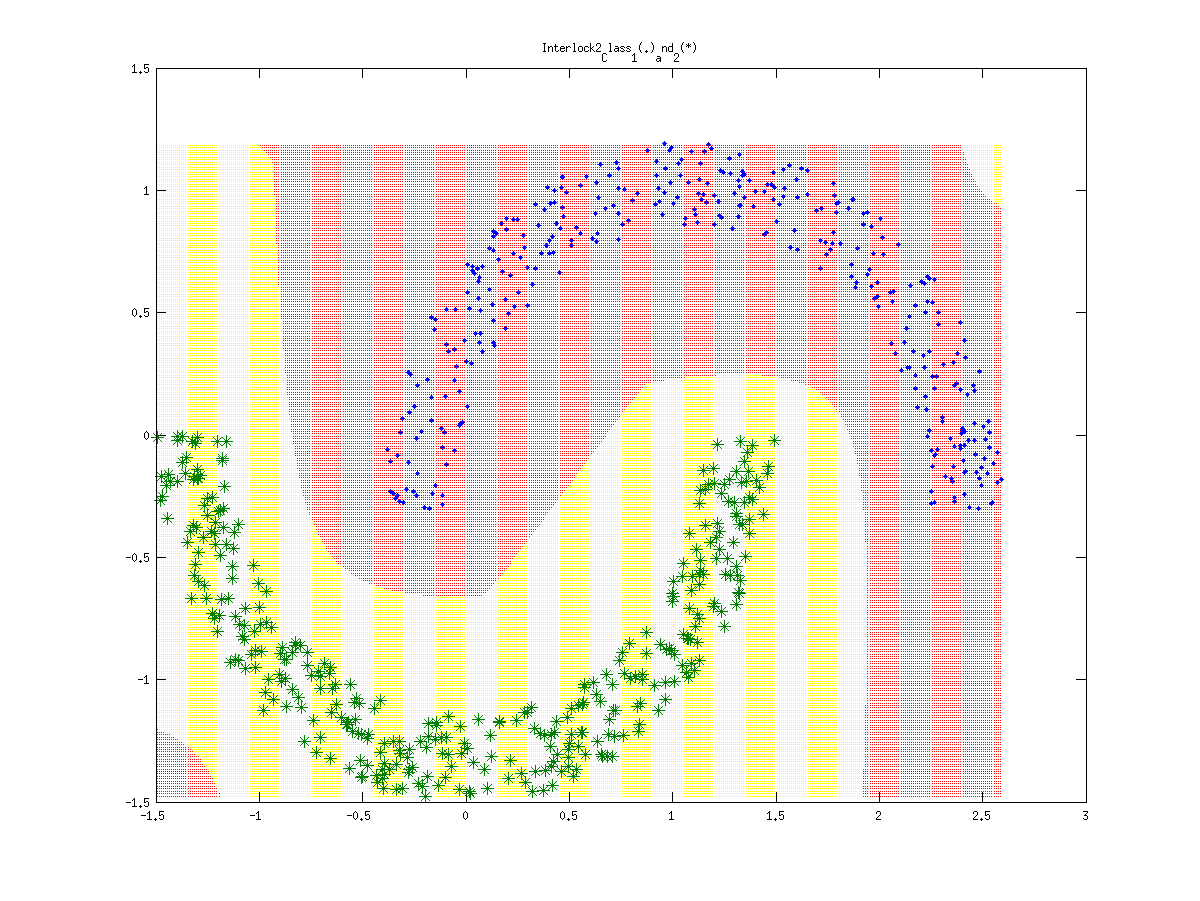
\includegraphics[width=\textwidth]{Interlock2.png}
		  	\captionof{figure}{ Decision region plot with the 
		  	training data} % [4]
		  \label{gfx/image}	
		\end{minipage}
		\begin{minipage}[t]{0.2\linewidth} % [2]
		\vspace{10pt} % [3]
			Correct   : 250	\\
			Incorrect : 0	\\
			Accuracy  : 100.00 \\
		\begin{center}
			\begin{tabular}{ |c|c|c|c| }
			\hline
			& & \multicolumn{2}{| c |}{Predicted} \\
			\hline
			& & Class 1 & Class 2 \\
			\hline
			\multirow{2}{*}{\rotatebox[origin=c]{90}{Act.}} & Class 1 & 125 & 0\\
			& Class 2 & 0 & 125\\
			
			\hline
			\end{tabular}
			\end{center}
		\end{minipage}
        
	 \subsubsection{4 clusters components}
     4 clusters per each class gives 8 gaussian distribution which have spreads in different directions. The upper peak on the distribution determines the class for that region so giving out 8 intersection decision boundary surfaces for gaussian distributions.
     
		\begin{minipage}[t]{0.6\linewidth}
			\vspace{0pt} % [3]
			 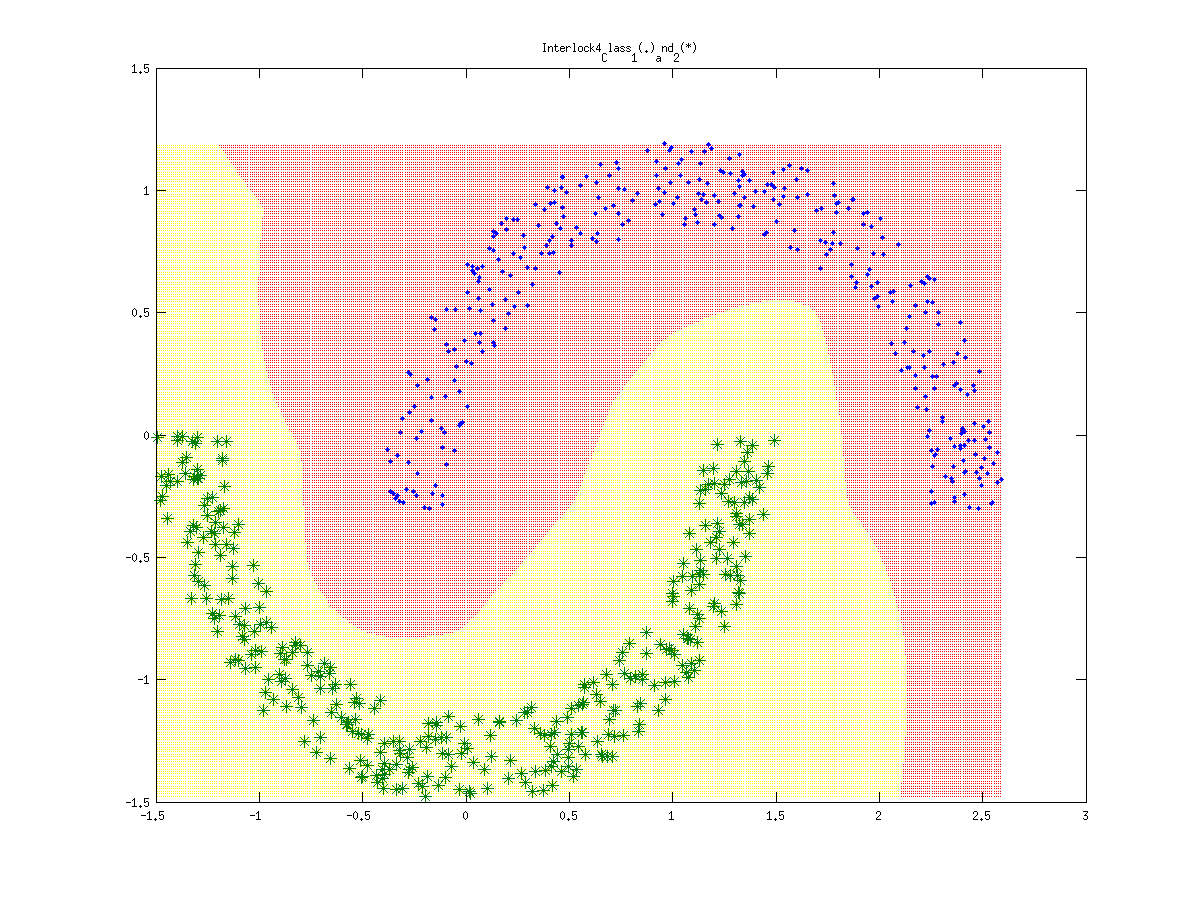
\includegraphics[width=\textwidth]{Interlock4.png}
		  	\captionof{figure}{ Decision region plot with the 
		  	training data.} % [4]
		  \label{gfx/image}	
		\end{minipage}
		\begin{minipage}[t]{0.2\linewidth} % [2]
		\vspace{10pt} % [3]
			Correct   : 250	\\
			Incorrect : 0	\\
			Accuracy  : 100.00 \\
		\begin{center}
			\begin{tabular}{ |c|c|c|c| }
			\hline
			& & \multicolumn{2}{| c |}{Predicted} \\
			\hline
			& & Class 1 & Class 2 \\
			\hline
			\multirow{2}{*}{\rotatebox[origin=c]{90}{Act.}} & Class 1 & 125 & 0\\
			& Class 2 & 0 & 125\\
			
			\hline
			\end{tabular}
			\end{center}
		\end{minipage}
        
        \subsubsection{8 clusters components}
        8 clusters per each class gives 16 gaussian distribution which have spreads in different directions. The upper peak on the distribution determines the class for that region so giving out 16 intersection decision boundary surfaces for gaussian distributions.
        
		\begin{minipage}[t]{0.6\linewidth}
			\vspace{0pt} % [3]
			 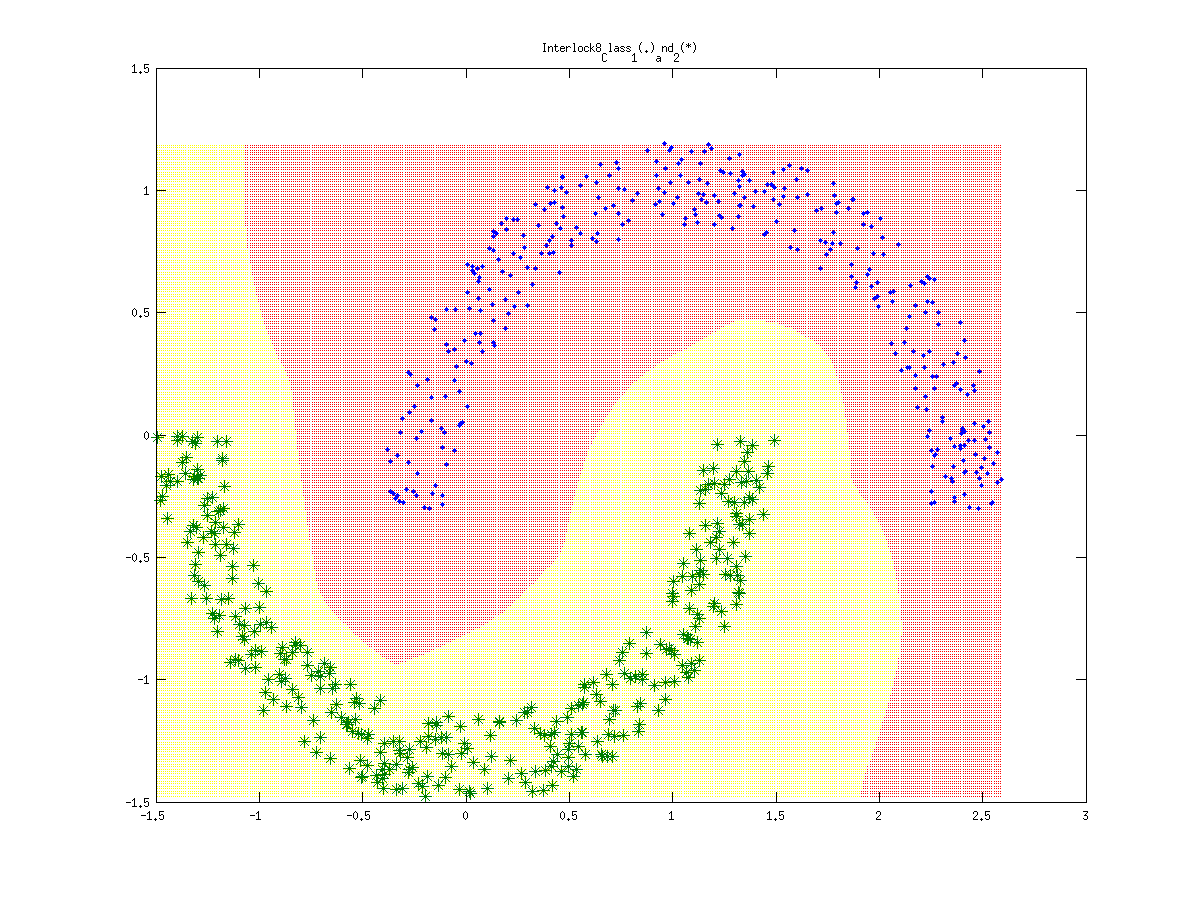
\includegraphics[width=\textwidth]{Interlock8.png}
		  	\captionof{figure}{ Decision region plot with the 
		  	training data.} % [4]
		  \label{gfx/image}	
		\end{minipage}
		\begin{minipage}[t]{0.2\linewidth} % [2]
		\vspace{10pt} % [3]
			Correct   : 250	\\
			Incorrect : 0	\\
			Accuracy  : 100.00 \\
		\begin{center}
			\begin{tabular}{ |c|c|c|c| }
			\hline
			& & \multicolumn{2}{| c |}{Predicted} \\
			\hline
			& & Class 1 & Class 2 \\
			\hline
			\multirow{2}{*}{\rotatebox[origin=c]{90}{Act.}} & Class 1 & 125 & 0\\
			& Class 2 & 0 & 125\\
			
			\hline
			\end{tabular}
			\end{center}
		\end{minipage}
	\subsection{Ring Data Set} 
		Ring data set includes 2 classes, both with same mean and with different covariances.
        
       \subsubsection{2 clusters components}
       2 clusters per each class gives 4 gaussian distribution which have spreads of different magnitude. The upper peak, class 1 peaks of the distribution determines the regions for center region giving out 3 intersection surfaces for gaussian distributions.
       
		\begin{minipage}[t]{0.6\linewidth}
			\vspace{0pt} % [3]
			 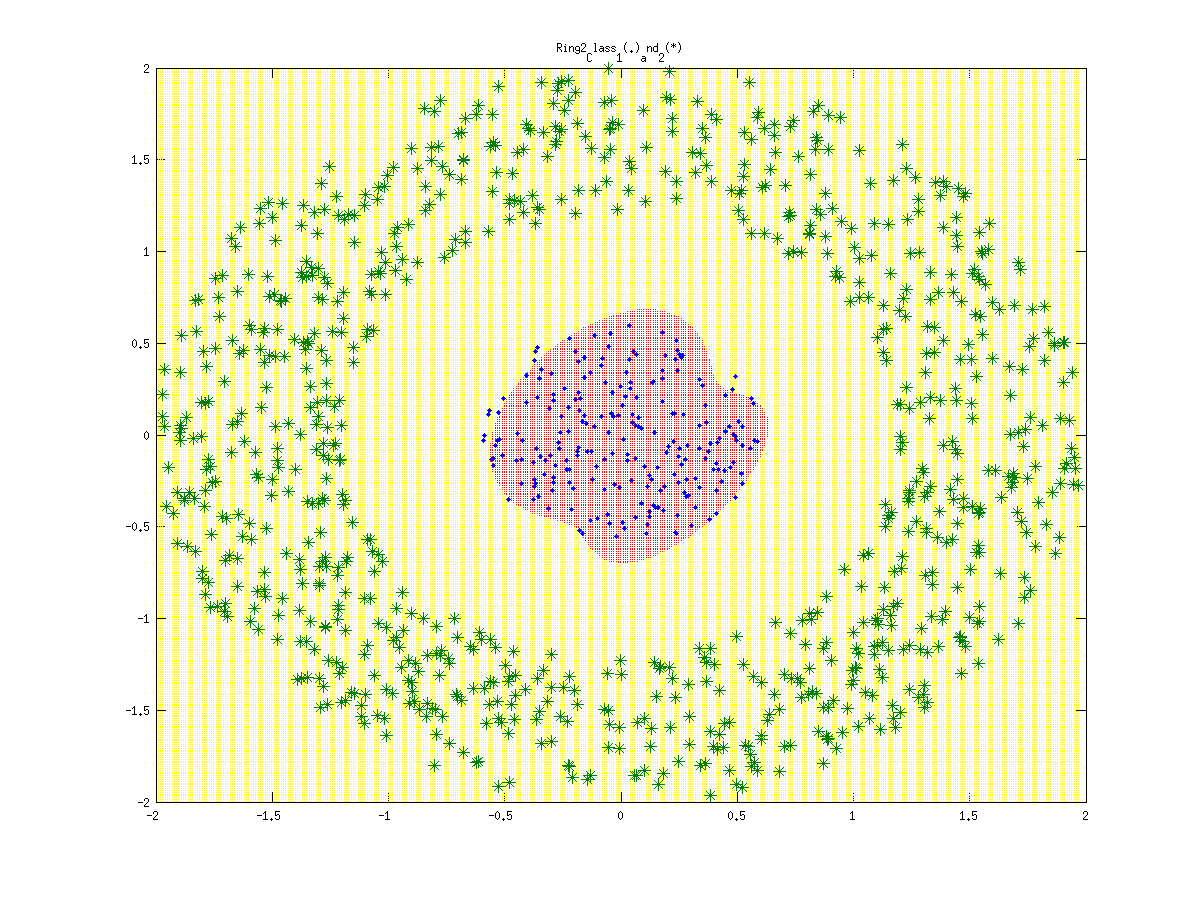
\includegraphics[width=\textwidth]{Ring2.png}
		  	\captionof{figure}{ Decision region plot with the 
		  	training data.} % [4]
		  \label{gfx/image}	
		\end{minipage}
		\begin{minipage}[t]{0.2\linewidth} % [2]
		\vspace{10pt} % [3]
			Correct   : 369	\\
			Incorrect : 6	\\
			Accuracy  : 98.4 \\
		\begin{center}
			\begin{tabular}{ |c|c|c|c| }
			\hline
			& & \multicolumn{2}{| c |}{Predicted} \\
			\hline
			& & Class 1 & Class 2 \\
			\hline
			\multirow{2}{*}{\rotatebox[origin=c]{90}{Act.}} & Class 1 & 69 & 6\\
			& Class 2 & 0 & 300\\
			
			\hline
			\end{tabular}
			\end{center}
		\end{minipage}
        
	 \subsubsection{4 clusters components}
     4 clusters per each class gives 8 gaussian distribution which have spreads of different magnitude. The upper peak, class 1 peaks of the distribution determines the regions for centre region giving out 5 intersection surfaces for gaussian distributions.
     
		\begin{minipage}[t]{0.6\linewidth}
			\vspace{0pt} % [3]
			 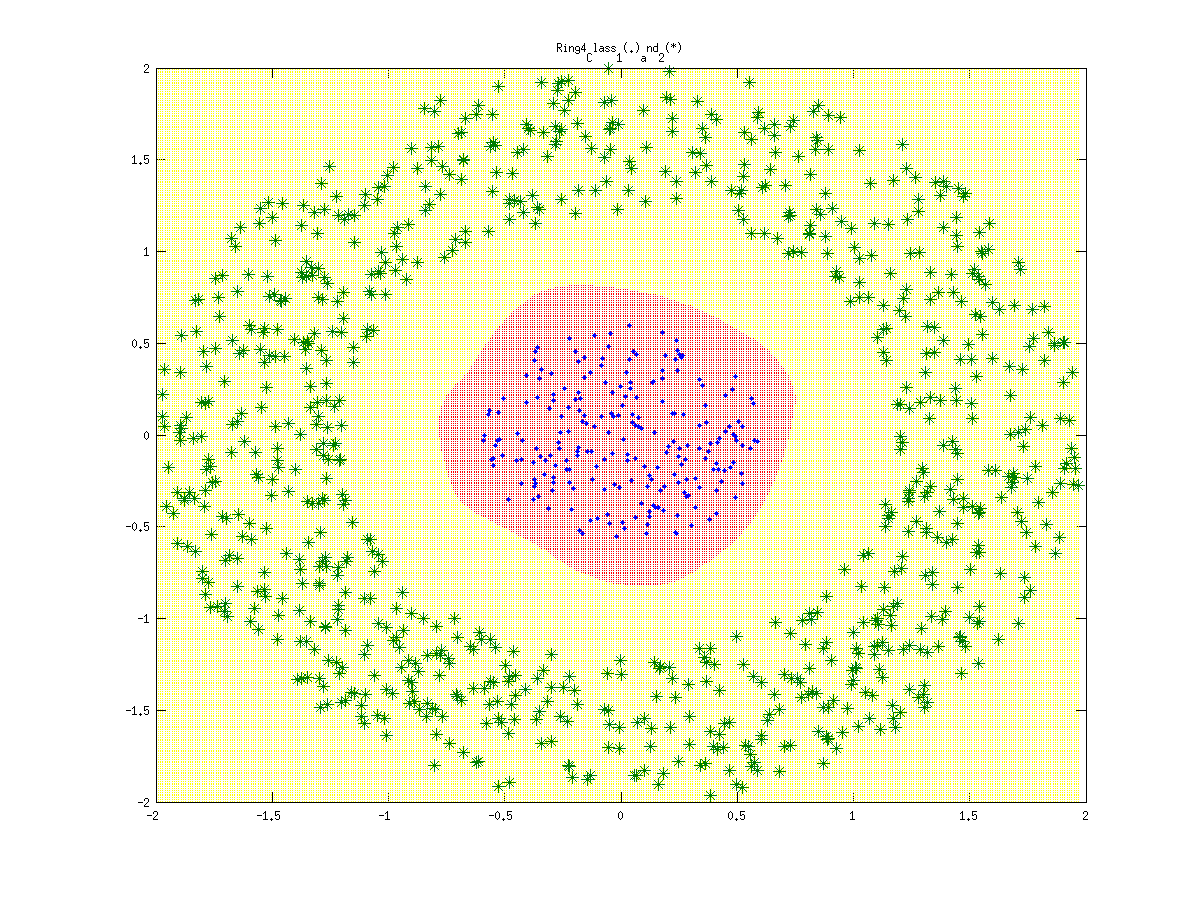
\includegraphics[width=\textwidth]{Ring4.png}
		  	\captionof{figure}{ Decision region plot with the 
		  	training data.} % [4]
		  \label{gfx/image}	
		\end{minipage}
		\begin{minipage}[t]{0.2\linewidth} % [2]
		\vspace{10pt} % [3]
			Correct   : 375	\\
			Incorrect : 0	\\
			Accuracy  : 100.00 \\
		\begin{center}
			\begin{tabular}{ |c|c|c|c| }
			\hline
			& & \multicolumn{2}{| c |}{Predicted} \\
			\hline
			& & Class 1 & Class 2 \\
			\hline
			\multirow{2}{*}{\rotatebox[origin=c]{90}{Act.}} & Class 1 & 75 & 0\\
			& Class 2 & 0 & 300\\
			
			\hline
			\end{tabular}
			\end{center}
		\end{minipage}
        
        \subsubsection{8 clusters components}
        8 clusters per each class gives 16 gaussian distribution which have spreads of different magnitude. The upper peak, class 1 peaks of the distribution determines the regions for center region giving out  intersection surfaces for gaussian distributions.
        
		\begin{minipage}[t]{0.6\linewidth}
			\vspace{0pt} % [3]
			 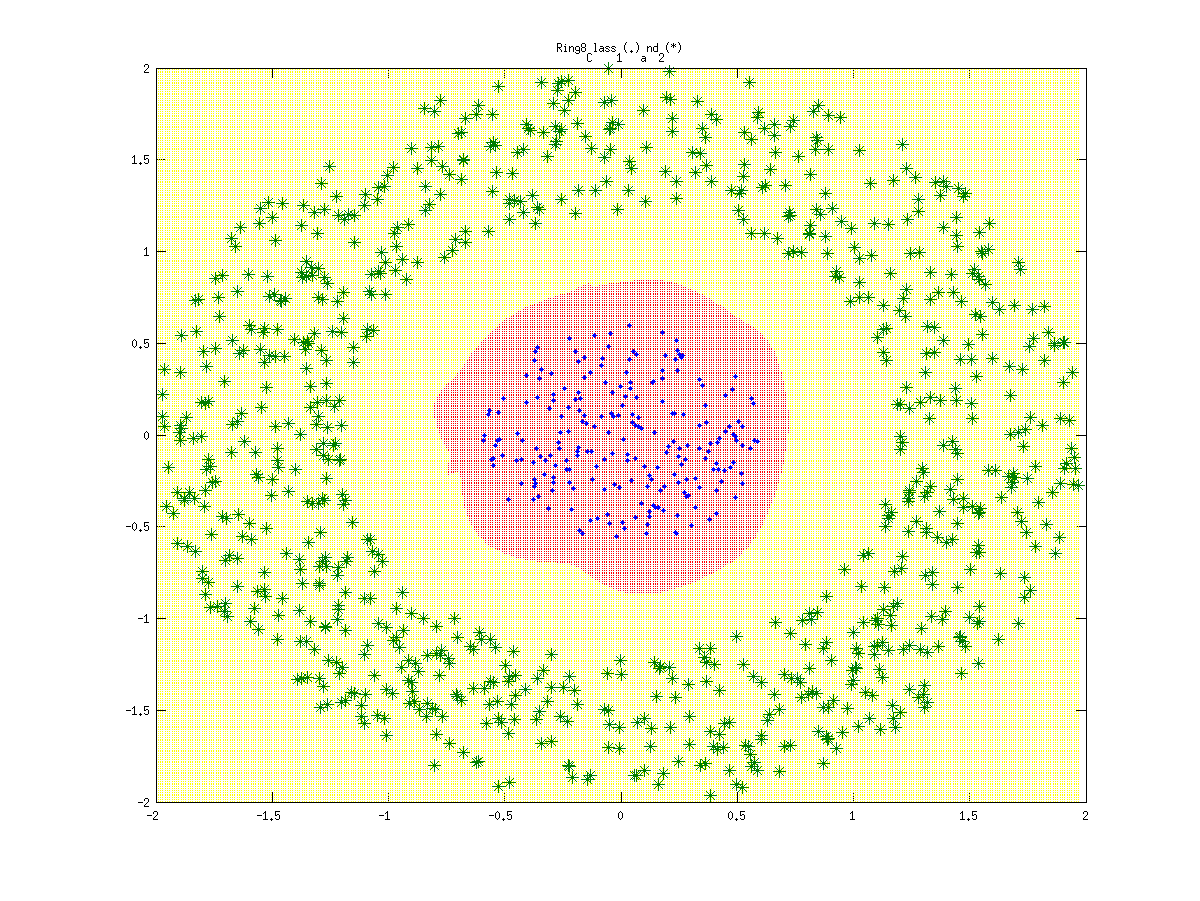
\includegraphics[width=\textwidth]{Ring8.png}
		  	\captionof{figure}{ Decision region plot with the 
		  	training data.} % [4]
		  \label{gfx/image}	
		\end{minipage}
		\begin{minipage}[t]{0.2\linewidth} % [2]
		\vspace{10pt} % [3]
			Correct   : 375	\\
			Incorrect : 0	\\
			Accuracy  : 100.00 \\
		\begin{center}
			\begin{tabular}{ |c|c|c|c| }
			\hline
			& & \multicolumn{2}{| c |}{Predicted} \\
			\hline
			& & Class 1 & Class 2 \\
			\hline
			\multirow{2}{*}{\rotatebox[origin=c]{90}{Act.}} & Class 1 & 75 & 0\\
			& Class 2 & 0 & 300\\
			
			\hline
			\end{tabular}
			\end{center}
		\end{minipage}	 
	
    	\subsection{Spiral Data Set} 
		Spiral data set contains 2 classes in form of spirals having slightly seperated mean and similar covariances.
        
       \subsubsection{2 clusters components}
       2 clusters for each class gives 4 gaussian distribution. The intersection of gaussian distribution for those clusters gives out the decision boundaries.
       
		\begin{minipage}[t]{0.6\linewidth}
			\vspace{0pt} % [3]
			 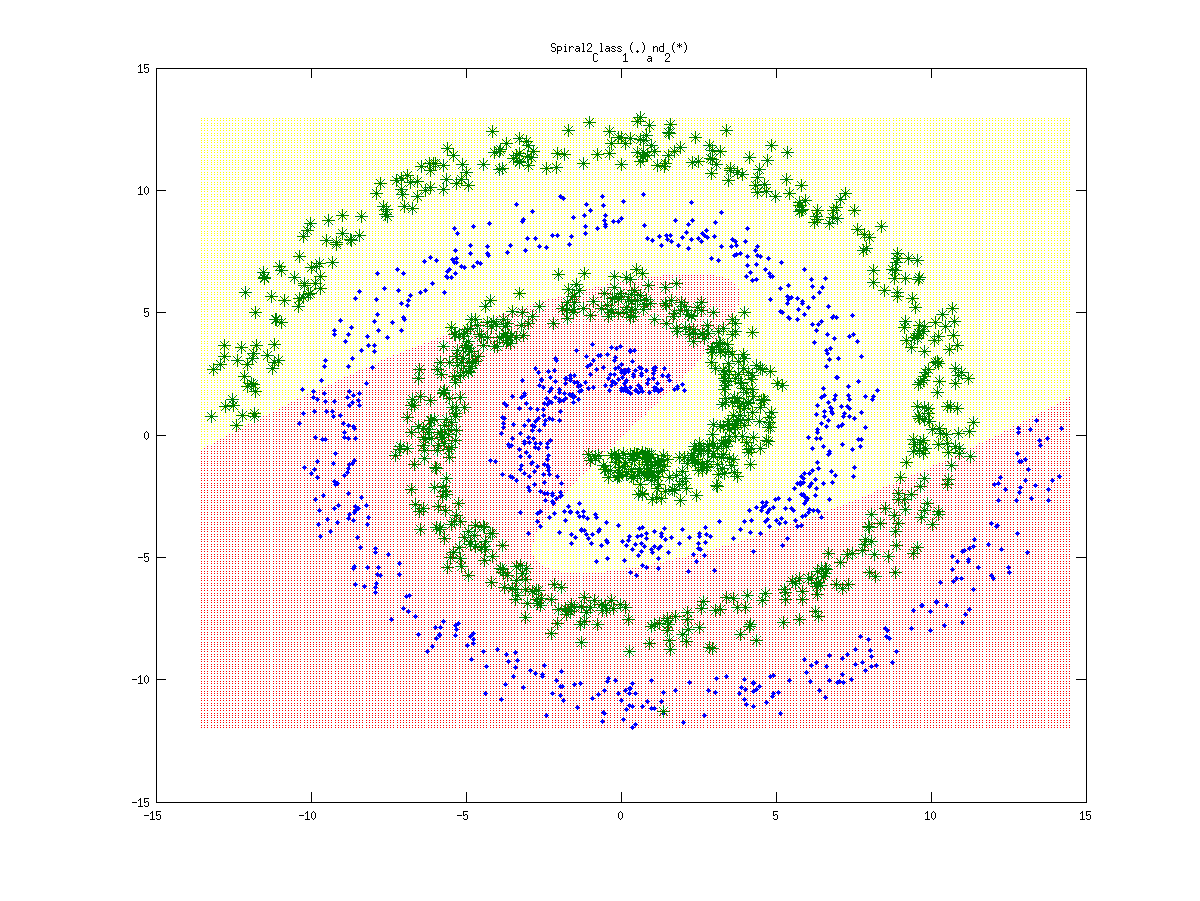
\includegraphics[width=\textwidth]{Spiral2.png}
		  	\captionof{figure}{ Decision region plot with the 
		  	training data.} % [4]
		  \label{gfx/image}	
		\end{minipage}
		\begin{minipage}[t]{0.2\linewidth} % [2]
		\vspace{10pt} % [3]
			Correct   : 400	\\
			Incorrect : 252	\\
			Accuracy  : 61.34 \\
		\begin{center}
			\begin{tabular}{ |c|c|c|c| }
			\hline
			& & \multicolumn{2}{| c |}{Predicted} \\
			\hline
			& & Class 1 & Class 2 \\
			\hline
			\multirow{2}{*}{\rotatebox[origin=c]{90}{Act.}} & Class 1 & 200 & 126\\
			& Class 2 & 126 & 200\\
			
			\hline
			\end{tabular}
			\end{center}
		\end{minipage}
        
	 \subsubsection{4 clusters components}	
     4 clusters for each class gives 8 gaussian distribution. The intersection of gaussian distribution for those clusters gives out the decision boundaries.
     
     	\begin{minipage}[t]{0.6\linewidth}
			\vspace{0pt} % [3]
			 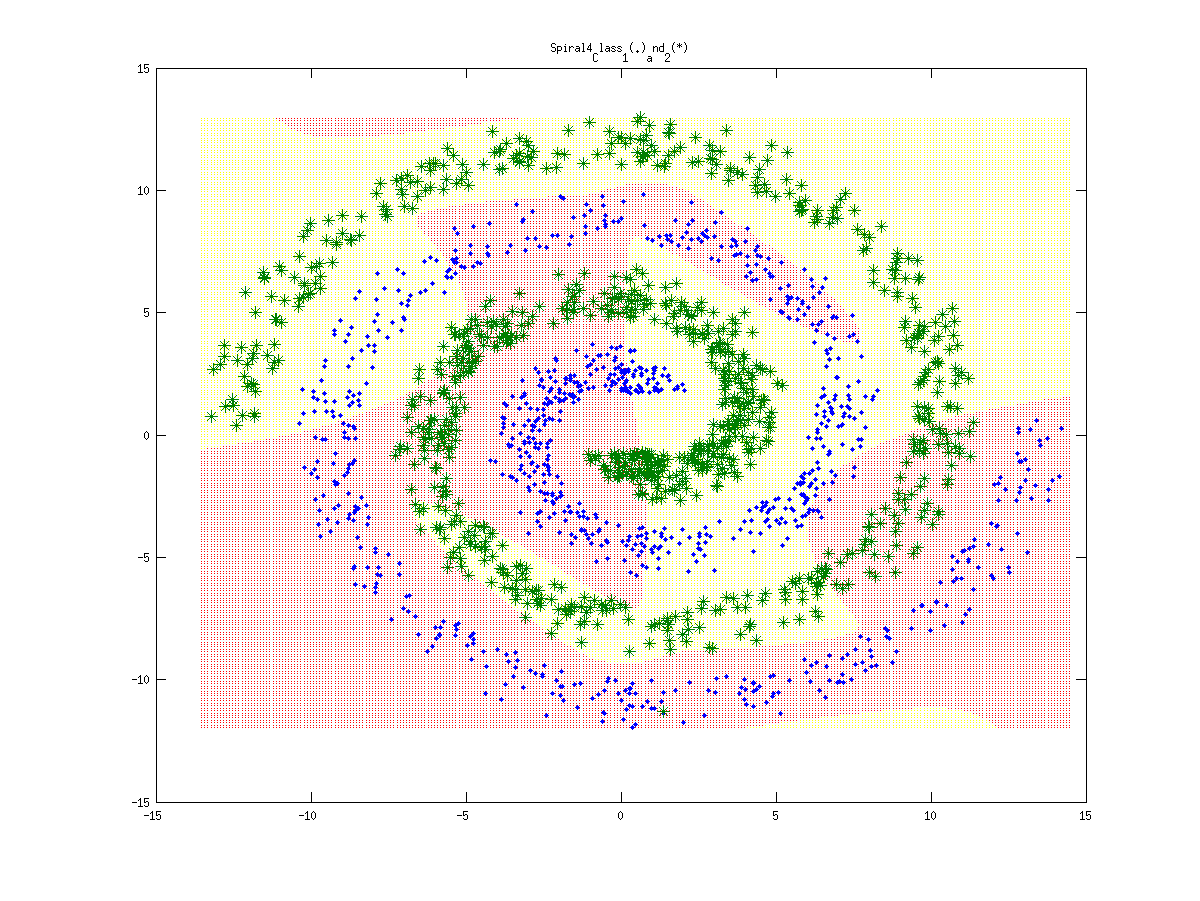
\includegraphics[width=\textwidth]{Spiral4.png}
		  	\captionof{figure}{ Decision region plot with the 
		  	training data.} % [4]
		  \label{gfx/image}	
		\end{minipage}
		\begin{minipage}[t]{0.6\linewidth}
			\vspace{10pt} % [3]
			Correct   : 449	\\
			Incorrect : 203	\\
			Accuracy  : 68.865 \\
		\begin{center}
			\begin{tabular}{ |c|c|c|c| }
			\hline
			& & \multicolumn{2}{| c |}{Predicted} \\
			\hline
			& & Class 1 & Class 2 \\
			\hline
			\multirow{2}{*}{\rotatebox[origin=c]{90}{Act.}} & Class 1 & 224 & 102\\
			& Class 2 & 101 & 225\\
			
			\hline
			\end{tabular}
			\end{center}
        \end{minipage}
        
        \subsubsection{8 clusters components}	
        8 clusters for each class gives 16 gaussian distribution. The intersection of gaussian distribution for those clusters gives out the decision boundaries. 
        
			\begin{minipage}[t]{0.6\linewidth}
			\vspace{0pt} % [3]
			 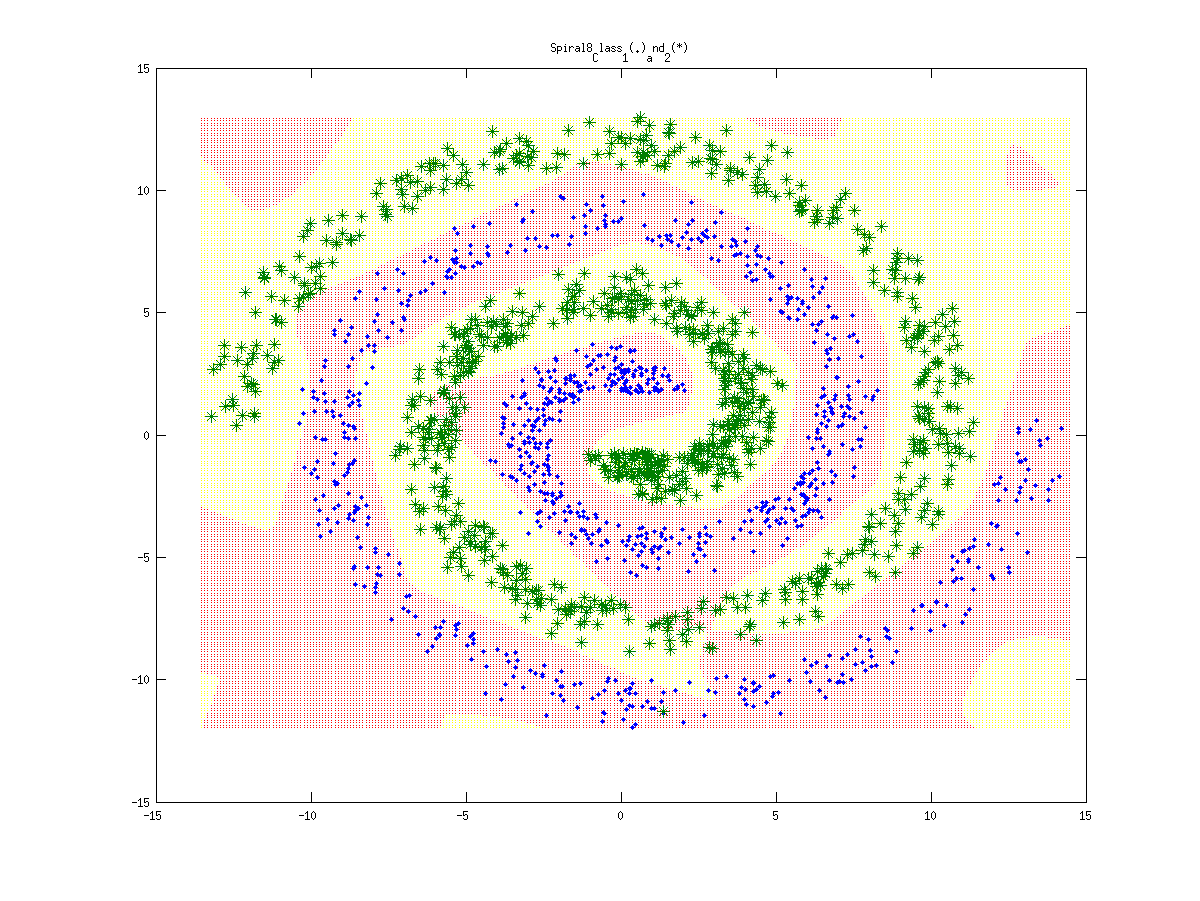
\includegraphics[width=\textwidth]{Spiral8.png}
		  	\captionof{figure}{ Decision region plot with the 
		  	training data.} % [4]
		  \label{gfx/image}	
		\end{minipage}
        \begin{minipage}[t]{0.6\linewidth}
		\vspace{10pt} % [3]
			Correct   : 641	\\
			Incorrect : 11	\\
			Accuracy  : 98.31 \\
		\begin{center}
			\begin{tabular}{ |c|c|c|c| }
			\hline
			& & \multicolumn{2}{| c |}{Predicted} \\
			\hline
			& & Class 1 & Class 2 \\
			\hline
			\multirow{2}{*}{\rotatebox[origin=c]{90}{Act.}} & Class 1 & 319 & 7\\
			& Class 126 & 4 & 322\\
			
			\hline
			\end{tabular}
			\end{center}
           \end{minipage}
           \subsubsection{12 clusters components}	
           12 clusters for each class gives 16 gaussian distribution. The intersection of gaussian distribution for those clusters gives out the decision boundaries. Interesting thing to note is 100 percent accuracy for this case.
		
			\begin{minipage}[t]{0.6\linewidth}
			\vspace{0pt} % [3]
			 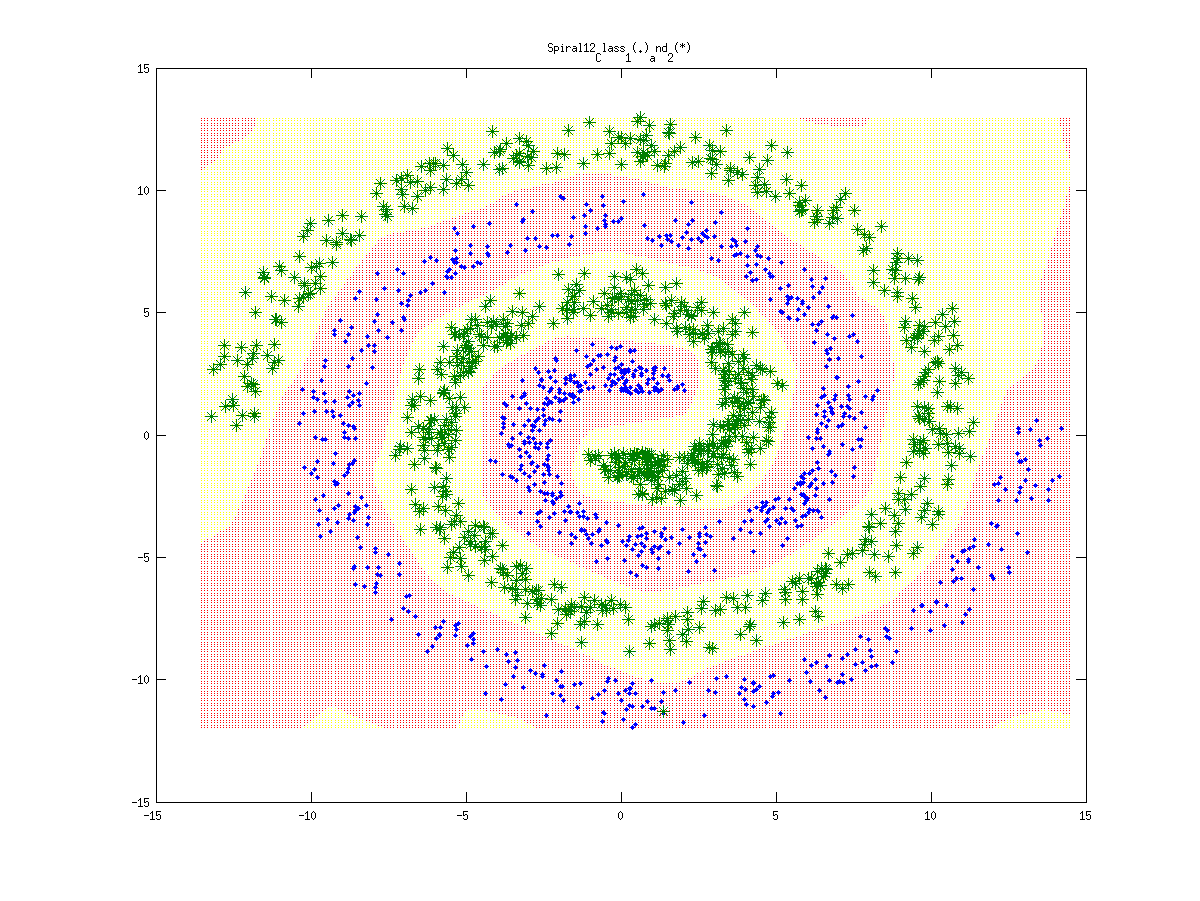
\includegraphics[width=\textwidth]{Spiral12.png}
		  	\captionof{figure}{ Decision region plot with the 
		  	training data.} % [4]
		  \label{gfx/image}	
		\end{minipage}
        \begin{minipage}[t]{0.6\linewidth}
        \vspace{10pt} % [3]
			Correct   : 652	\\
			Incorrect : 0\\
			Accuracy  : 100.00 \\
		\begin{center}
			\begin{tabular}{ |c|c|c|c| }
			\hline
			& & \multicolumn{2}{| c |}{Predicted} \\
			\hline
			& & Class 1 & Class 2 \\
			\hline
			\multirow{2}{*}{\rotatebox[origin=c]{90}{Act.}} & Class 1 & 326 & 0\\
			& Class 126 & 0 & 326\\
			
			\hline
			\end{tabular}
			\end{center}
           \end{minipage} 
		\subsection{Real World Data Set} 
		
       \subsubsection{2 clusters components}	
		We assume two cluster components for each class i.e. 
two gaussian distributions for a class. The green data points on bottom left corner are not classified correctly because the two distributions center in the region between the pink and blue class, and hence could not classify the green points at corner.

        \begin{minipage}[t]{0.6\linewidth}
			\vspace{0pt} % [3]
			 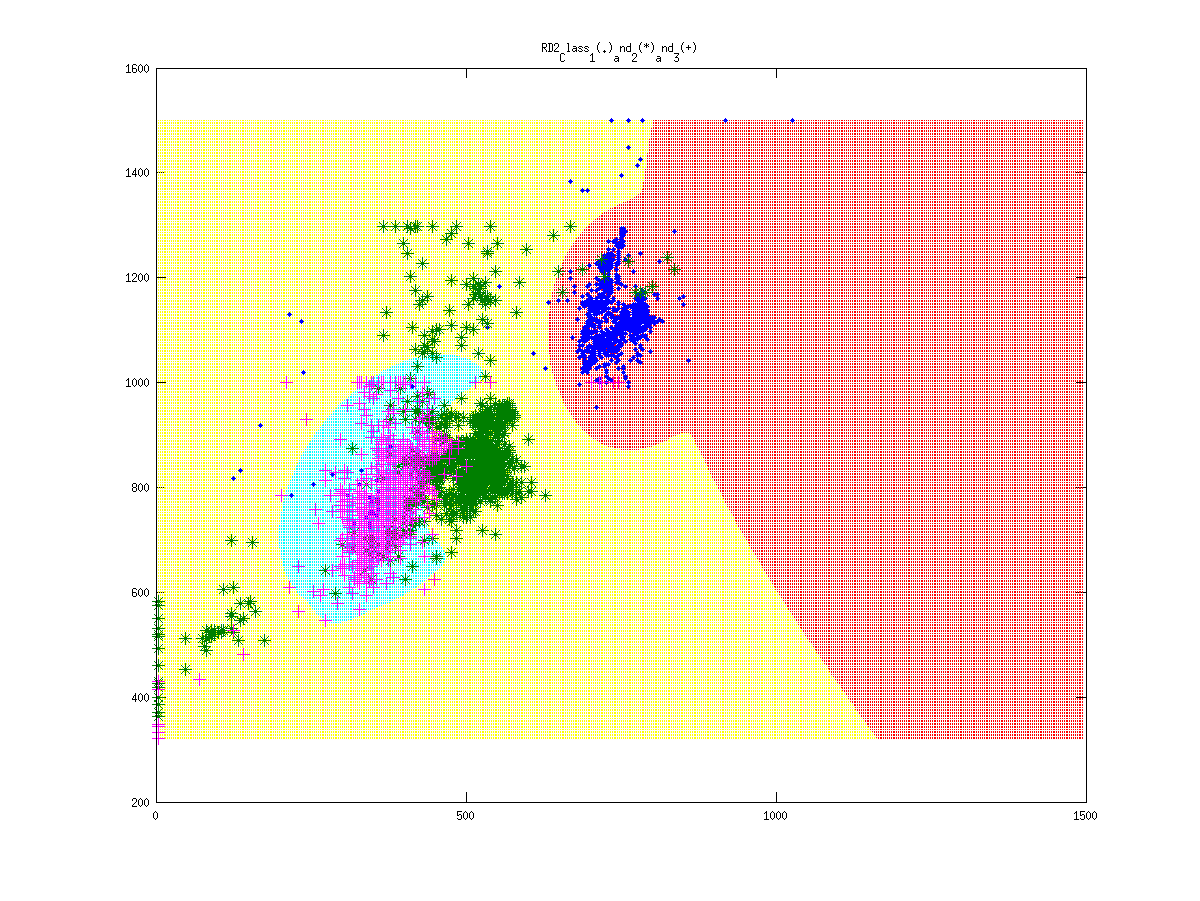
\includegraphics[width=\textwidth]{RD2.png}
		  	\captionof{figure}{ Decision region plot with the 
		  	training data.} % [4]
		  \label{gfx/image}	
		\end{minipage}
		\begin{minipage}[t]{0.2\linewidth} % [2]
		\vspace{10pt} % [3]
			Correct   : 1494	\\
			Incorrect : 284	\\
			Accuracy  : 84.026 \\
		\begin{center}
			\begin{tabular}{ |c|c|c|c|c| }
			\hline
			& & \multicolumn{3}{| c |}{Predicted} \\
			\hline
			& & Class 1 & Class 2 & Class 3\\
			\hline
			\multirow{3}{*}{\rotatebox[origin=c]{90}{Act.}} & Class 1 & 506 & 18 & 17\\
			& Class 2 & 1 & 419 & 193\\
			& Class 3 & 5 & 50 & 567\\
			\hline
			\end{tabular}
			\end{center}
		\end{minipage}
        
	 \subsubsection{4 clusters components}	
     	The green points are classified correctly because of two more cluster peaks, which very well accommodate those. The region for blue points also expands as the one for yellow point class narrows. The blue class seems very well spread, probably because of large non diagonal covariance matrices.
        
		\begin{minipage}[t]{0.6\linewidth}
			\vspace{0pt} % [3]
			 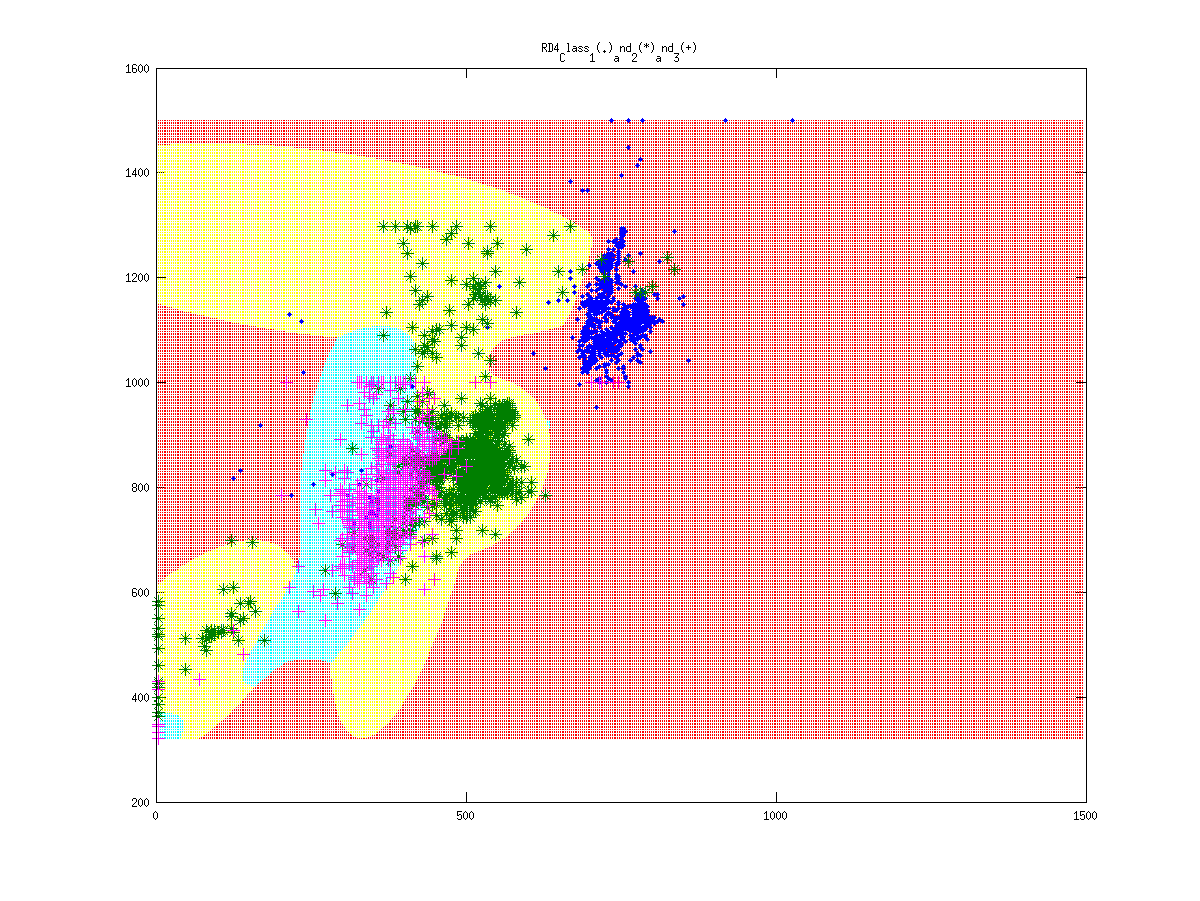
\includegraphics[width=\textwidth]{RD4.png}
		  	\captionof{figure}{ Decision region plot with the 
		  	training data.} % [4]
		  \label{gfx/image}	
		\end{minipage}
		\begin{minipage}[t]{0.2\linewidth} % [2]
		\vspace{10pt} % [3]
			Correct   : 1453	\\
			Incorrect : 325\\
			Accuracy  : 81.721 \\
		\begin{center}
			\begin{tabular}{ |c|c|c|c|c| }
			\hline
			& & \multicolumn{3}{| c |}{Predicted} \\
			\hline
			& & Class 1 & Class 2 & Class 3\\
			\hline
			\multirow{3}{*}{\rotatebox[origin=c]{90}{Act.}} & Class 1 & 512 & 14 & 15\\
			& Class 2 & 4 & 368 & 241\\
			& Class 3 & 12 & 37 & 573\\
			\hline
			\end{tabular}
			\end{center}
		\end{minipage}
        
        \subsubsection{8 clusters components}	
        Adding more clusters for each class makes the surfaces more precise and narrow. This is because of the increased probability for the data point to be in the respective clusters of the assigned class.
        
		\begin{minipage}[t]{0.6\linewidth}
			\vspace{0pt} % [3]
			 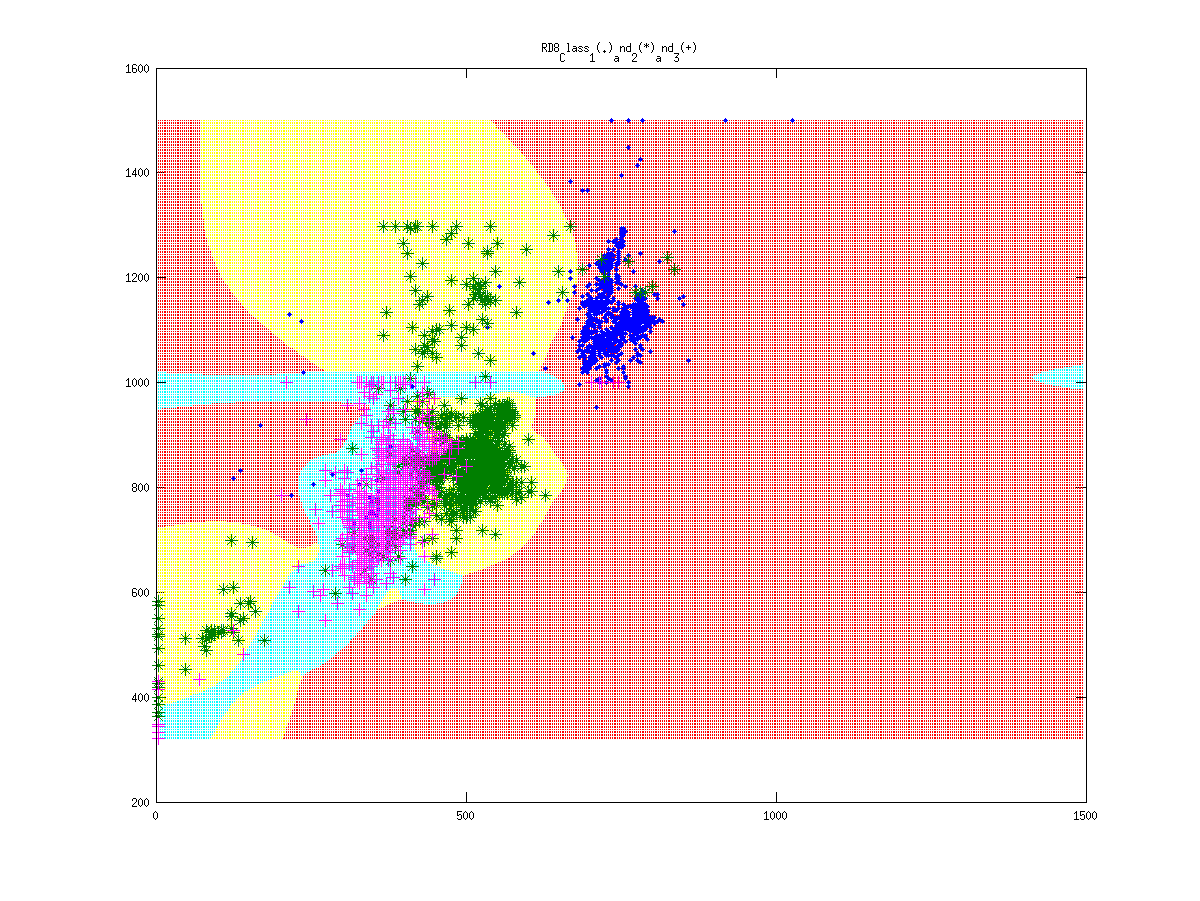
\includegraphics[width=\textwidth]{RD8.png}
		  	\captionof{figure}{ Decision region plot with the 
		  	training data.} % [4]
		  \label{gfx/image}	
		\end{minipage}
		\begin{minipage}[t]{0.2\linewidth} % [2]
		\vspace{10pt} % [3]
			Correct   : 1533	\\
			Incorrect : 245	\\
			Accuracy  : 86.220 \\
		\begin{center}
			\begin{tabular}{ |c|c|c|c|c| }
			\hline
			& & \multicolumn{3}{| c |}{Predicted} \\
			\hline
			& & Class 1 & Class 2 & Class 3\\
			\hline
			\multirow{3}{*}{\rotatebox[origin=c]{90}{Act.}} & Class 1 & 515 & 9 & 17\\
			& Class 2 & 2 & 437 & 174\\
			& Class 3 & 10 & 31 & 581\\
			\hline
			\end{tabular}
			\end{center}
		\end{minipage}	
        
        \subsection{Image Scene Data Set} 
       
       \begin{minipage}[t]{0.5\linewidth} % [2]
        \subsubsection{8 clusters components}	
		\vspace{10pt} % [3]
			Correct   : 213	\\
			Incorrect : 66	\\
			Accuracy  : 76.344 \\
		\begin{center}
			\begin{tabular}{ |c|c|c|c|c| }
			\hline
			& & \multicolumn{3}{| c |}{Predicted} \\
			\hline
			& & Class 1 & Class 2 & Class 3\\
			\hline
			\multirow{3}{*}{\rotatebox[origin=c]{90}{Act.}} & Class 1 & 68 & 10 & 4\\
			& Class 2 & 3 & 77 & 14\\
			& Class 3 & 12 & 23 & 63\\
			\hline
			\end{tabular}
			\end{center}
		\end{minipage}
        \begin{minipage}[t]{0.5\linewidth} % [2]
        \subsubsection{32 clusters components}	
		\vspace{10pt} % [3]
			Correct   : 374	\\
			Incorrect : 1	\\
			Accuracy  : 99.733 \\
		\begin{center}
			\begin{tabular}{ |c|c|c|c|c| }
			\hline
			& & \multicolumn{3}{| c |}{Predicted} \\
			\hline
			& & Class 1 & Class 2 & Class 3\\
			\hline
			\multirow{3}{*}{\rotatebox[origin=c]{90}{Act.}} & Class 1 & 125 & 0 & 0\\
			& Class 2 & 0 & 125 & 0\\
			& Class 3 & 0 & 1 & 124\\
			\hline
			\end{tabular}
			\end{center}
		\end{minipage}
        \begin{minipage}[t]{0.5\linewidth} % [1]     
        \vspace{10pt} % [1]
        \subsubsection{64 clusters components}	
		\vspace{10pt} % [1]
			Correct   : 1533	\\
			Incorrect : 245	\\
			Accuracy  : 86.220\\
		\begin{center}
			\begin{tabular}{ |c|c|c|c|c| }
			\hline
			& & \multicolumn{3}{| c |}{Predicted} \\
			\hline
			& & Class 1 & Class 2 & Class 3\\
			\hline
			\multirow{3}{*}{\rotatebox[origin=c]{90}{Act.}} & Class 1 & 125 & 0 & 0\\
			& Class 2 & 0 & 125 & 0\\
			& Class 3 & 0 & 1 & 124\\
			\hline
			\end{tabular}
			\end{center}
		\end{minipage}
         \begin{minipage}[t]{0.5\linewidth} % [2]  
         \vspace{10pt} % [1]
        \subsubsection{128 clusters components}	
		\vspace{10pt} % [2]
			Correct   : 374	\\
			Incorrect : 1	\\
			Accuracy  : 99.733 \\
		\begin{center}
			\begin{tabular}{ |c|c|c|c|c| }
			\hline
			& & \multicolumn{3}{| c |}{Predicted} \\
			\hline
			& & Class 1 & Class 2 & Class 3\\
			\hline
			\multirow{3}{*}{\rotatebox[origin=c]{90}{Act.}} & Class 1 & 125 & 0 & 0\\
			& Class 2 & 0 & 125 & 0\\
			& Class 3 & 0 & 1 & 124\\
			\hline
			\end{tabular}
			\end{center}
		\end{minipage}
         
\section{Conclusion}
	As per the observations, we can make the following conclusions :
	
	\begin{enumerate}
	  \item The Decision Boundaries are more accurate when we model the data as a mixture of multiple gaussian as compared to the a single gaussian.
	  \item Different results are obtained when number of clusters $k$ are varied.   	
	  \item The Decision Boundaries appears to be piece wise combination of quadratic boundaries as in case of unimodal gaussian case.
      \item Although the accuracy tends to increase with the number of clusters assumed for a class, but due to overlapping data, the over clustering may cause the class to cover non-belonging points as well, this is evident in the real world data 4 cluster and 2 cluster case.  
	\end{enumerate}

\end{document}
              
            